\section{Methane pyrolysis in shock-tube}

The pyrolysis of 5\% and 10\% $\mathrm{CH_4}$-Ar was investigated using a constant volume reactor model (CVR) for the post-shock temperature, $T_5$ range of 1800-3000 K, and pressure, $P_5$ range of 4.7-7.1 bar. $P_5$ was assumed to linearly increase with $T_5$ across the simulation cases. Caltech mechanism was used and the inception models were calibrated in order to match carbon yield at t=1.5 ms with the measurement~\citep{agafonov2016unified} using a dual-beam absorption–emission technique. \citet{agafonov2016unified} reported yield$\times$E(m) at $\mathrm{\lambda}$=632~nm, and yield data was retrieved using E(m)=0.37 suggested therein. 


\begin{figure}[H]
	\centering
	\begin{subfigure}[t]{0.4\textwidth}
		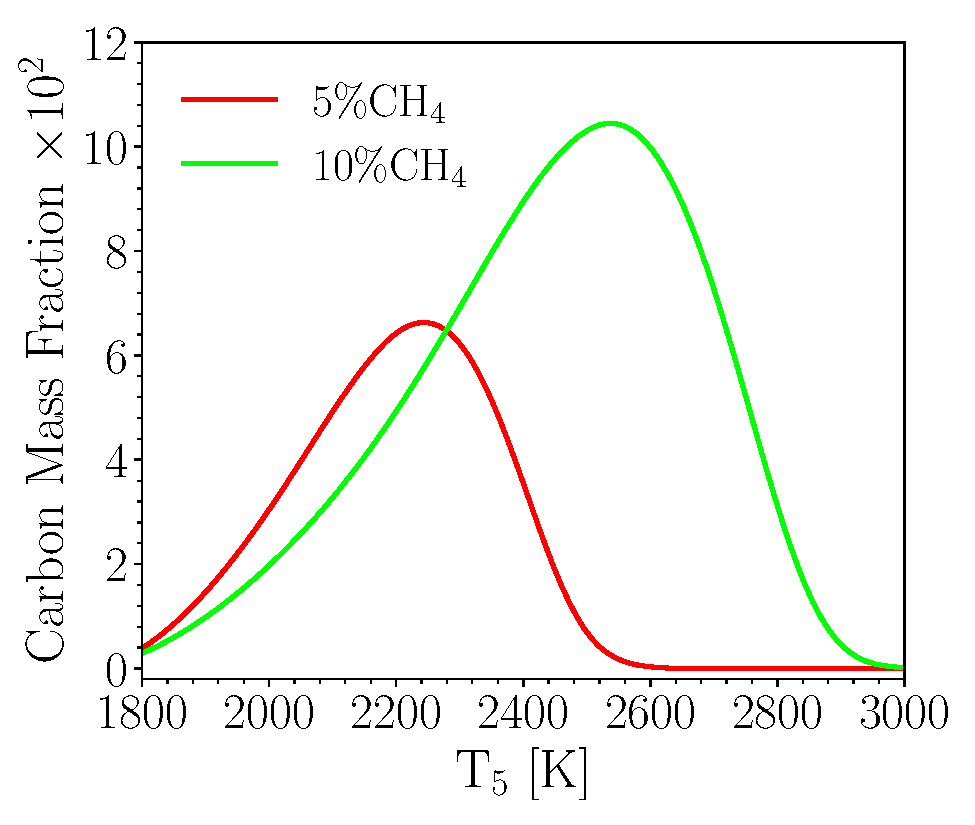
\includegraphics[width=1\textwidth]{Figures/Results/Shocktube/Agafonov2016/SPC_cmf.pdf}
	\end{subfigure}
	\begin{subfigure}[t]{0.4\textwidth}
		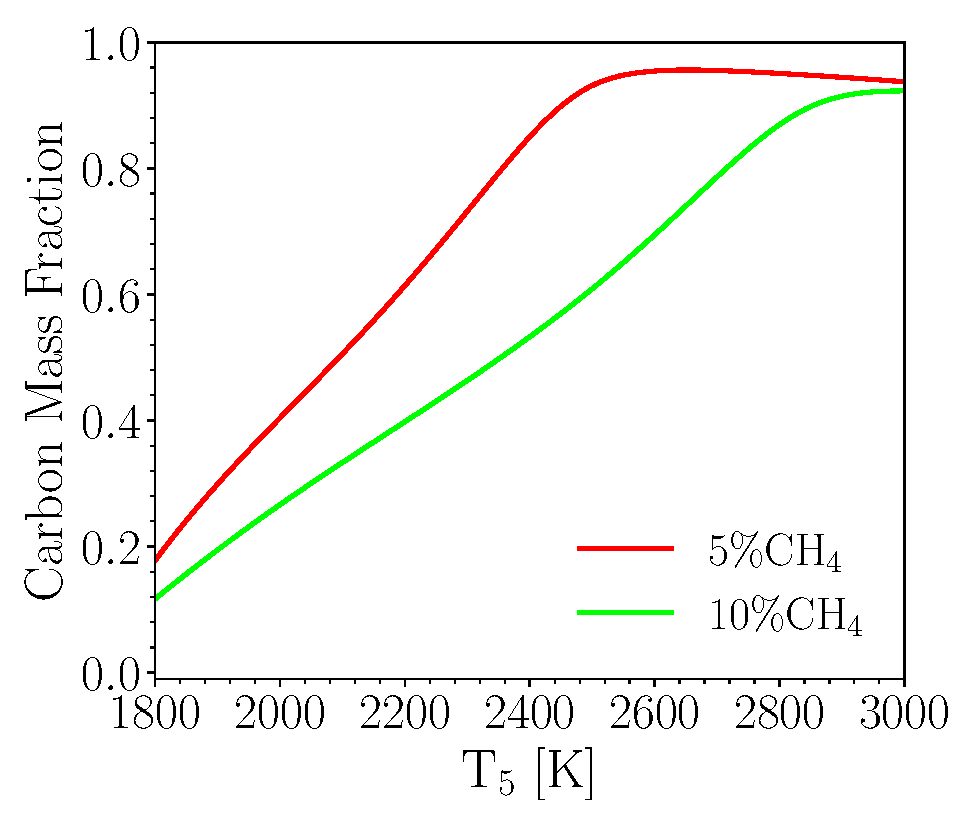
\includegraphics[width=1\textwidth]{Figures/Results/Shocktube/Agafonov2016/C2H2_cmf.pdf}
	\end{subfigure}
	\caption{The bell-shape temperature profile of carbon mass fraction of soot precursors (A2 and larger) combined (a) and $\mathrm{C_2H_2}$ (b) at t=1.5 ms during pyrolysis of 5\% (red line) and 10\%~$\mathrm{CH_4}$-Ar (green line) obtained using Caltech mechanism without considering soot}
	\label{fig:SPC_cmf} 
\end{figure}

Fig.~\ref{fig:SPC_cmf} shows that the carbon mass fraction (CMF) of soot precursors obtained using Caltech mechanism without considering soot formation exhibits a bell-shape profile highlighting that the similar temperature dependence of soot yield (volume fraction) mainly stems from PAH chemistry. Moreover, the temperature of peak CMF shifts to higher temperatures as methane mole fraction increase from 5 to 10\%.


\begin{figure}[H]
	\centering
	\begin{tikzpicture}
		\draw (0, 0) node[inner sep=0] 	{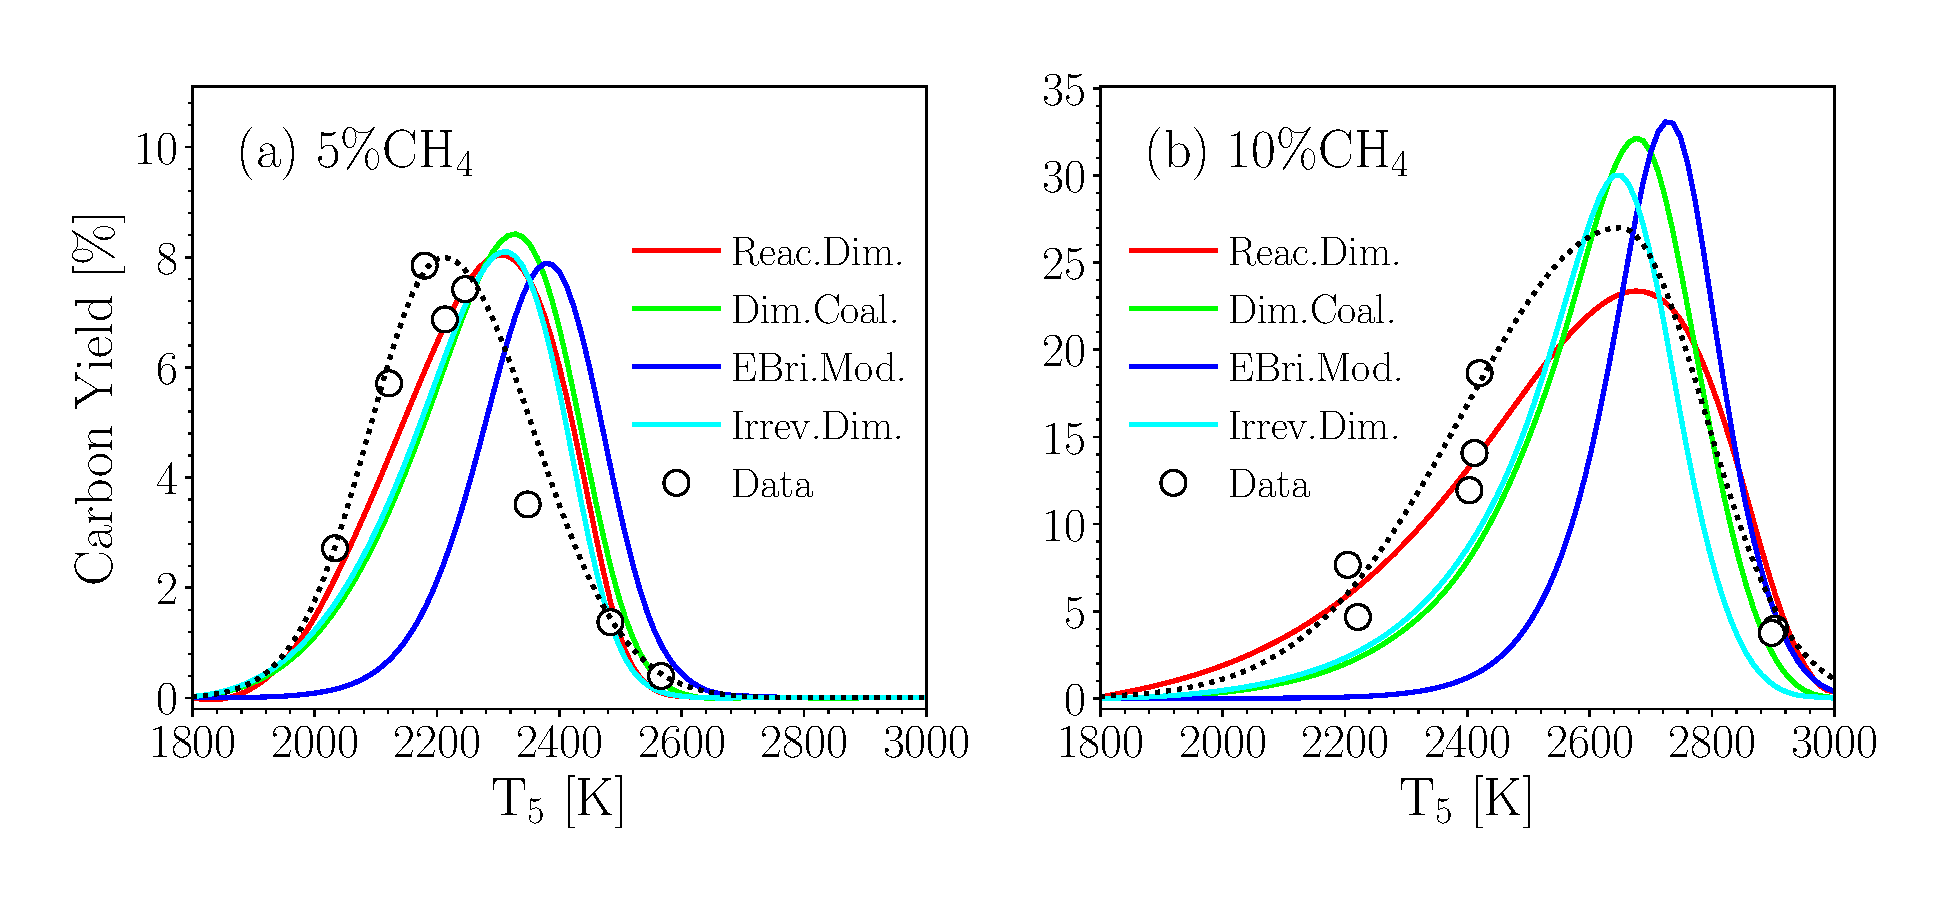
\includegraphics[width=0.8\textwidth]{Figures/Results/Shocktube/Agafonov2016/carbon_yield.pdf}};
		\draw (-0.68, -0.23) node {\scriptsize{\cite{agafonov2016unified}}};
		\draw (2.42, -0.23) node {\scriptsize{\cite{agafonov2016unified}}};
	\end{tikzpicture}
	\caption{The bell-shape temperature profile of soot carbon yield at t=1.5 ms for 5\% (a) and 10\%~$\mathrm{CH_4}$ (b) in Ar obtained using Caltech mechanism and different inception models calibrated to minimize the prediction with extinction measurements~\citep{agafonov2016unified}.}
	\label{fig:shockagof_yield} 
\end{figure}

Fig.~\ref{fig:shockagof_yield} shows soot carbon yield predicted using Caltech mechanism where inception flux and PAH adsorption rate were adjusted using a scaling factor (equal for the both) to minimize the prediction error compared to the data from extinction measurements~\citep{agafonov2016unified}. A skew exponential curve fit (represented by the black dotted line) was applied to illustrate the trend in soot yield and identify the temperature at which the yield likely reaches its maximum. The predicted temperature of peak yield is larger than peak of curve-fit in both $\mathrm{CH_4}$ concentrations by 100-200 K depending on the inception model. This difference is due the contribution of  HACA to surface growth that depends on $\mathrm{C_2H_2}$ concentration which increases with temperature.

\begin{figure}[H]
	\centering
	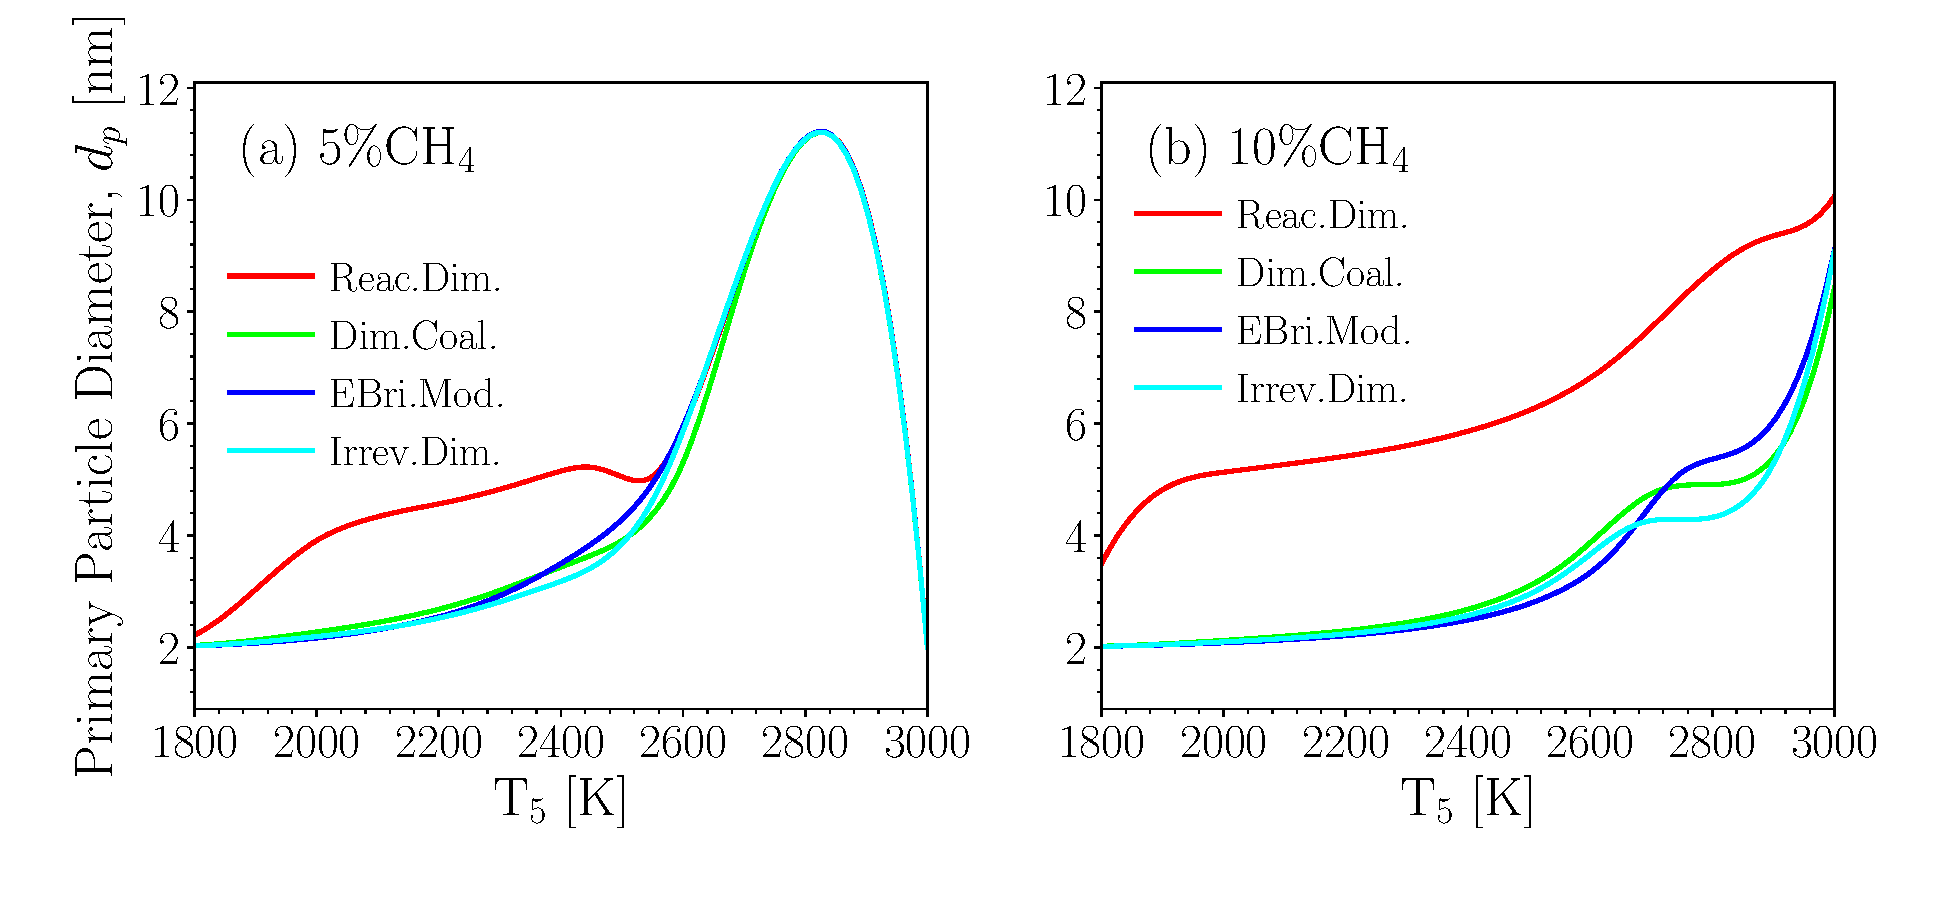
\includegraphics[width=0.8\textwidth]{Figures/Results/Shocktube/Agafonov2016/d_p.pdf}
	\caption{The temperature dependence of mean primary particle diameter, $d_p$ at t=1.5 ms for 5\% (a) and 10\%~$\mathrm{CH_4}$ (b) in Ar obtained using Caltech mechanism and different inception models calibrated to minimize the prediction with extinction measurements~\citep{agafonov2016unified}.}
	\label{fig:shockagof_dp} 
\end{figure}

Fig.\ref{fig:shockagof_dp} shows that $d_p$ increases with temperature up to 10 nm. For 5\% $\mathrm{CH_4}$, $d_p$ reaches the peak around 2800 K and drops quickly to 2 nm which is the minimum allowed diameter in the model. Reactive Dimerization results in overall larger primary particle diameters, but the behavior of the rest of inception models are similar.

\begin{figure}[H]
	\centering
	\begin{tikzpicture}
		\draw (0, 0) node[inner sep=0] 	{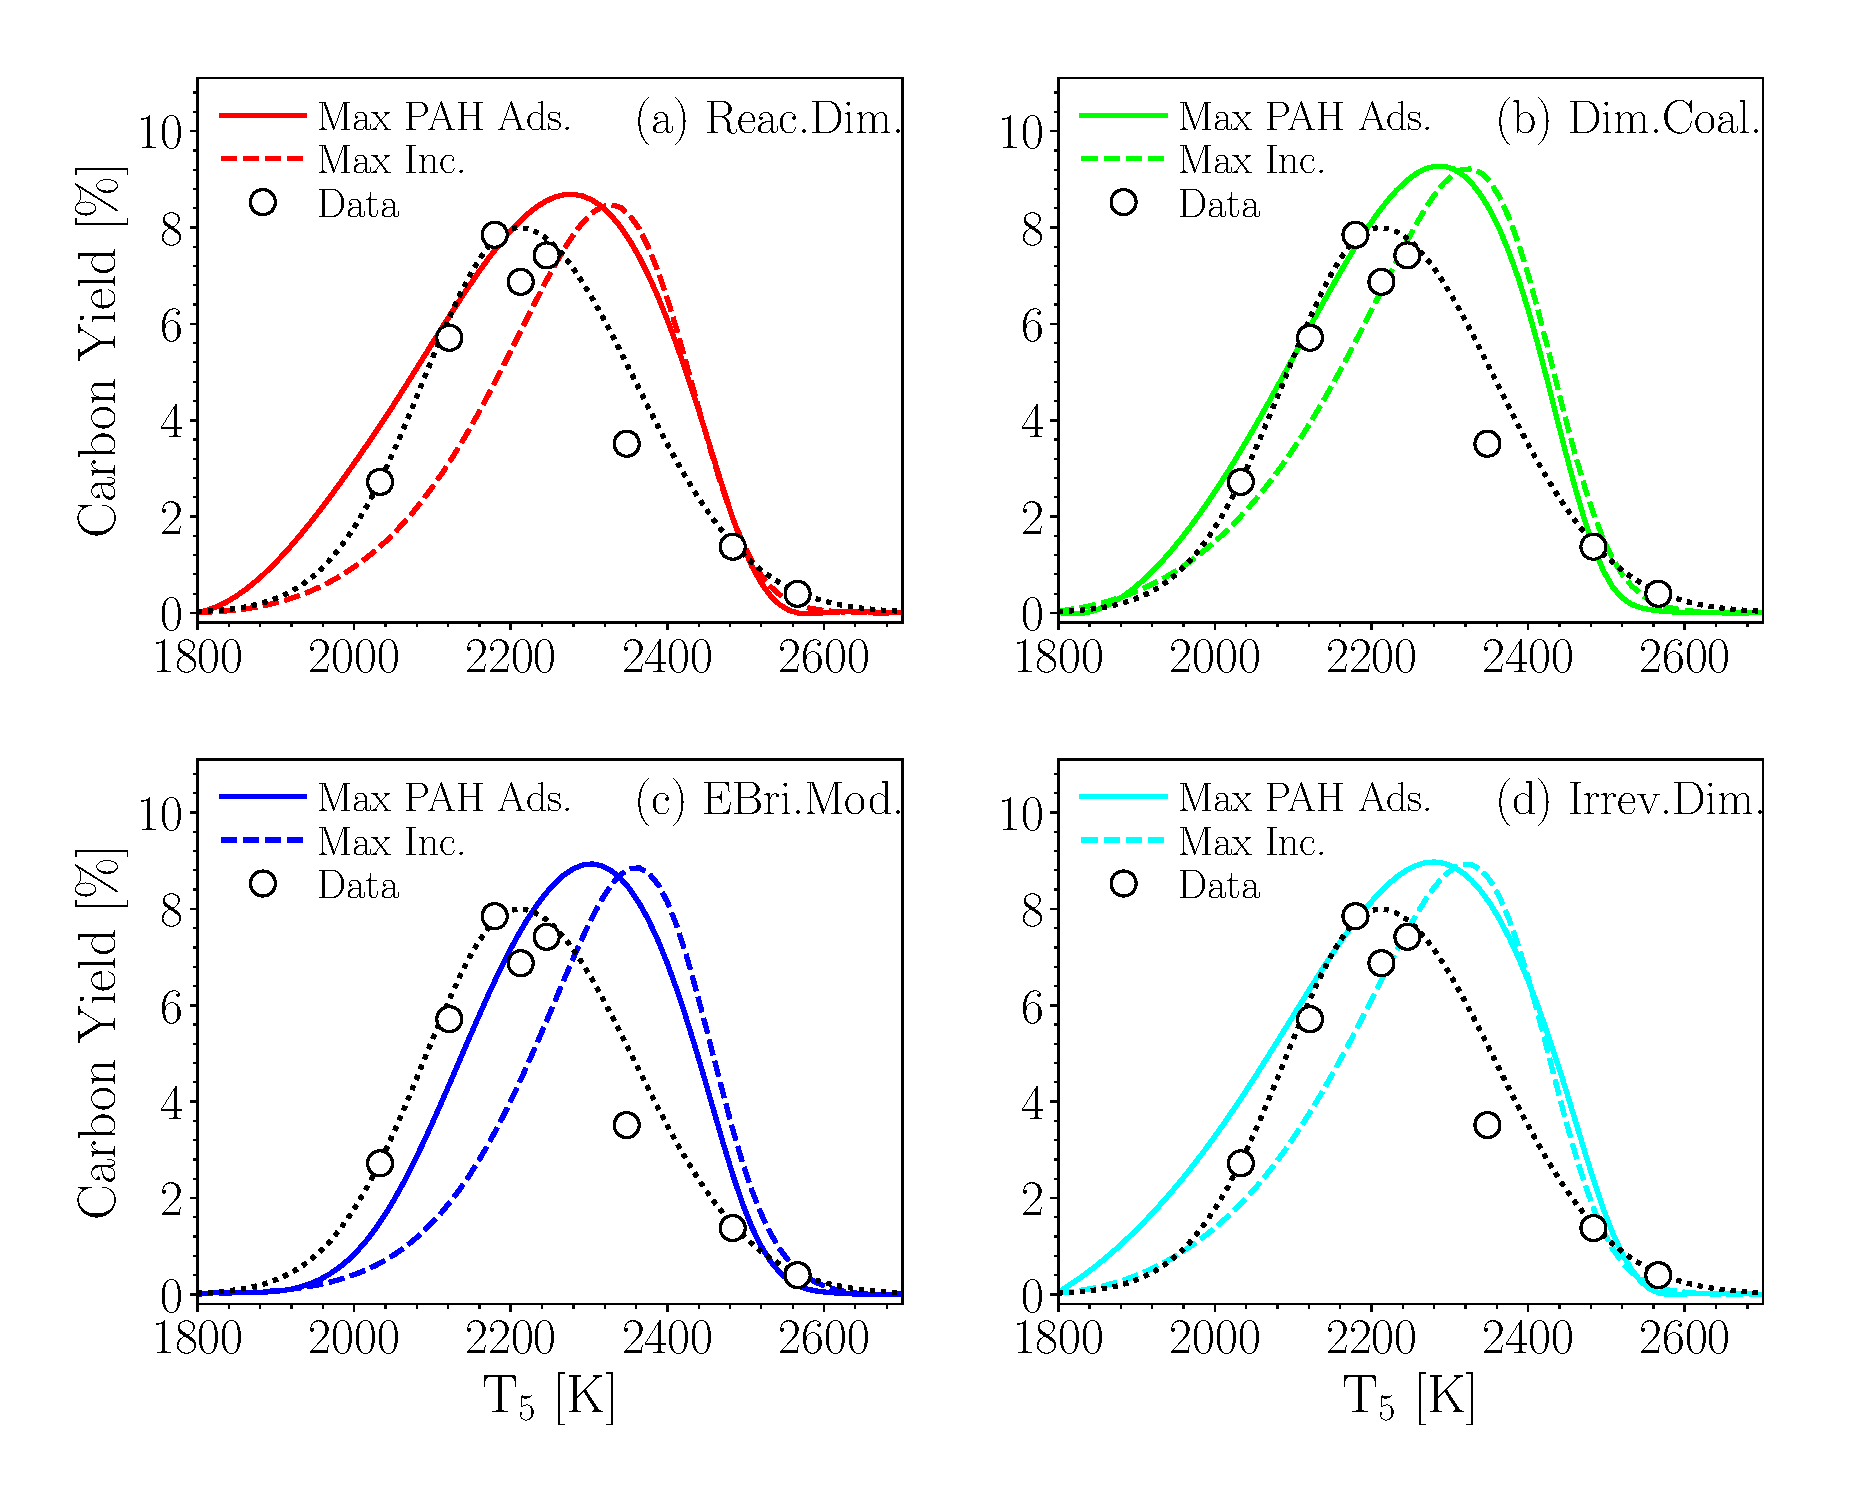
\includegraphics[width=0.8\textwidth]{Figures/Results/Shocktube/Agafonov2016/carbon_yield_maxincads.pdf}};
		\draw (-3.18, -0.9) node {\scriptsize{\cite{agafonov2016unified}}};
		\draw (2.46, -0.9) node {\scriptsize{\cite{agafonov2016unified}}};
		\draw (-3.18, 3.55) node {\scriptsize{\cite{agafonov2016unified}}};
		\draw (2.46, 3.55) node {\scriptsize{\cite{agafonov2016unified}}};
	\end{tikzpicture}
	\caption{The comparison of soot carbon yield at t=1.5 ms when maximum inception and PAH adsorption were applied to minimized the prediction  error compared to measurements~\citep{agafonov2016unified} for 5\% (a) and 10\%~$\mathrm{CH_4}$ (b) in Ar obtained using Caltech mechanism and different inception models.}
	\label{fig:shockagof_yield_maxincads} 
\end{figure}

\begin{figure}[H]
	\centering
	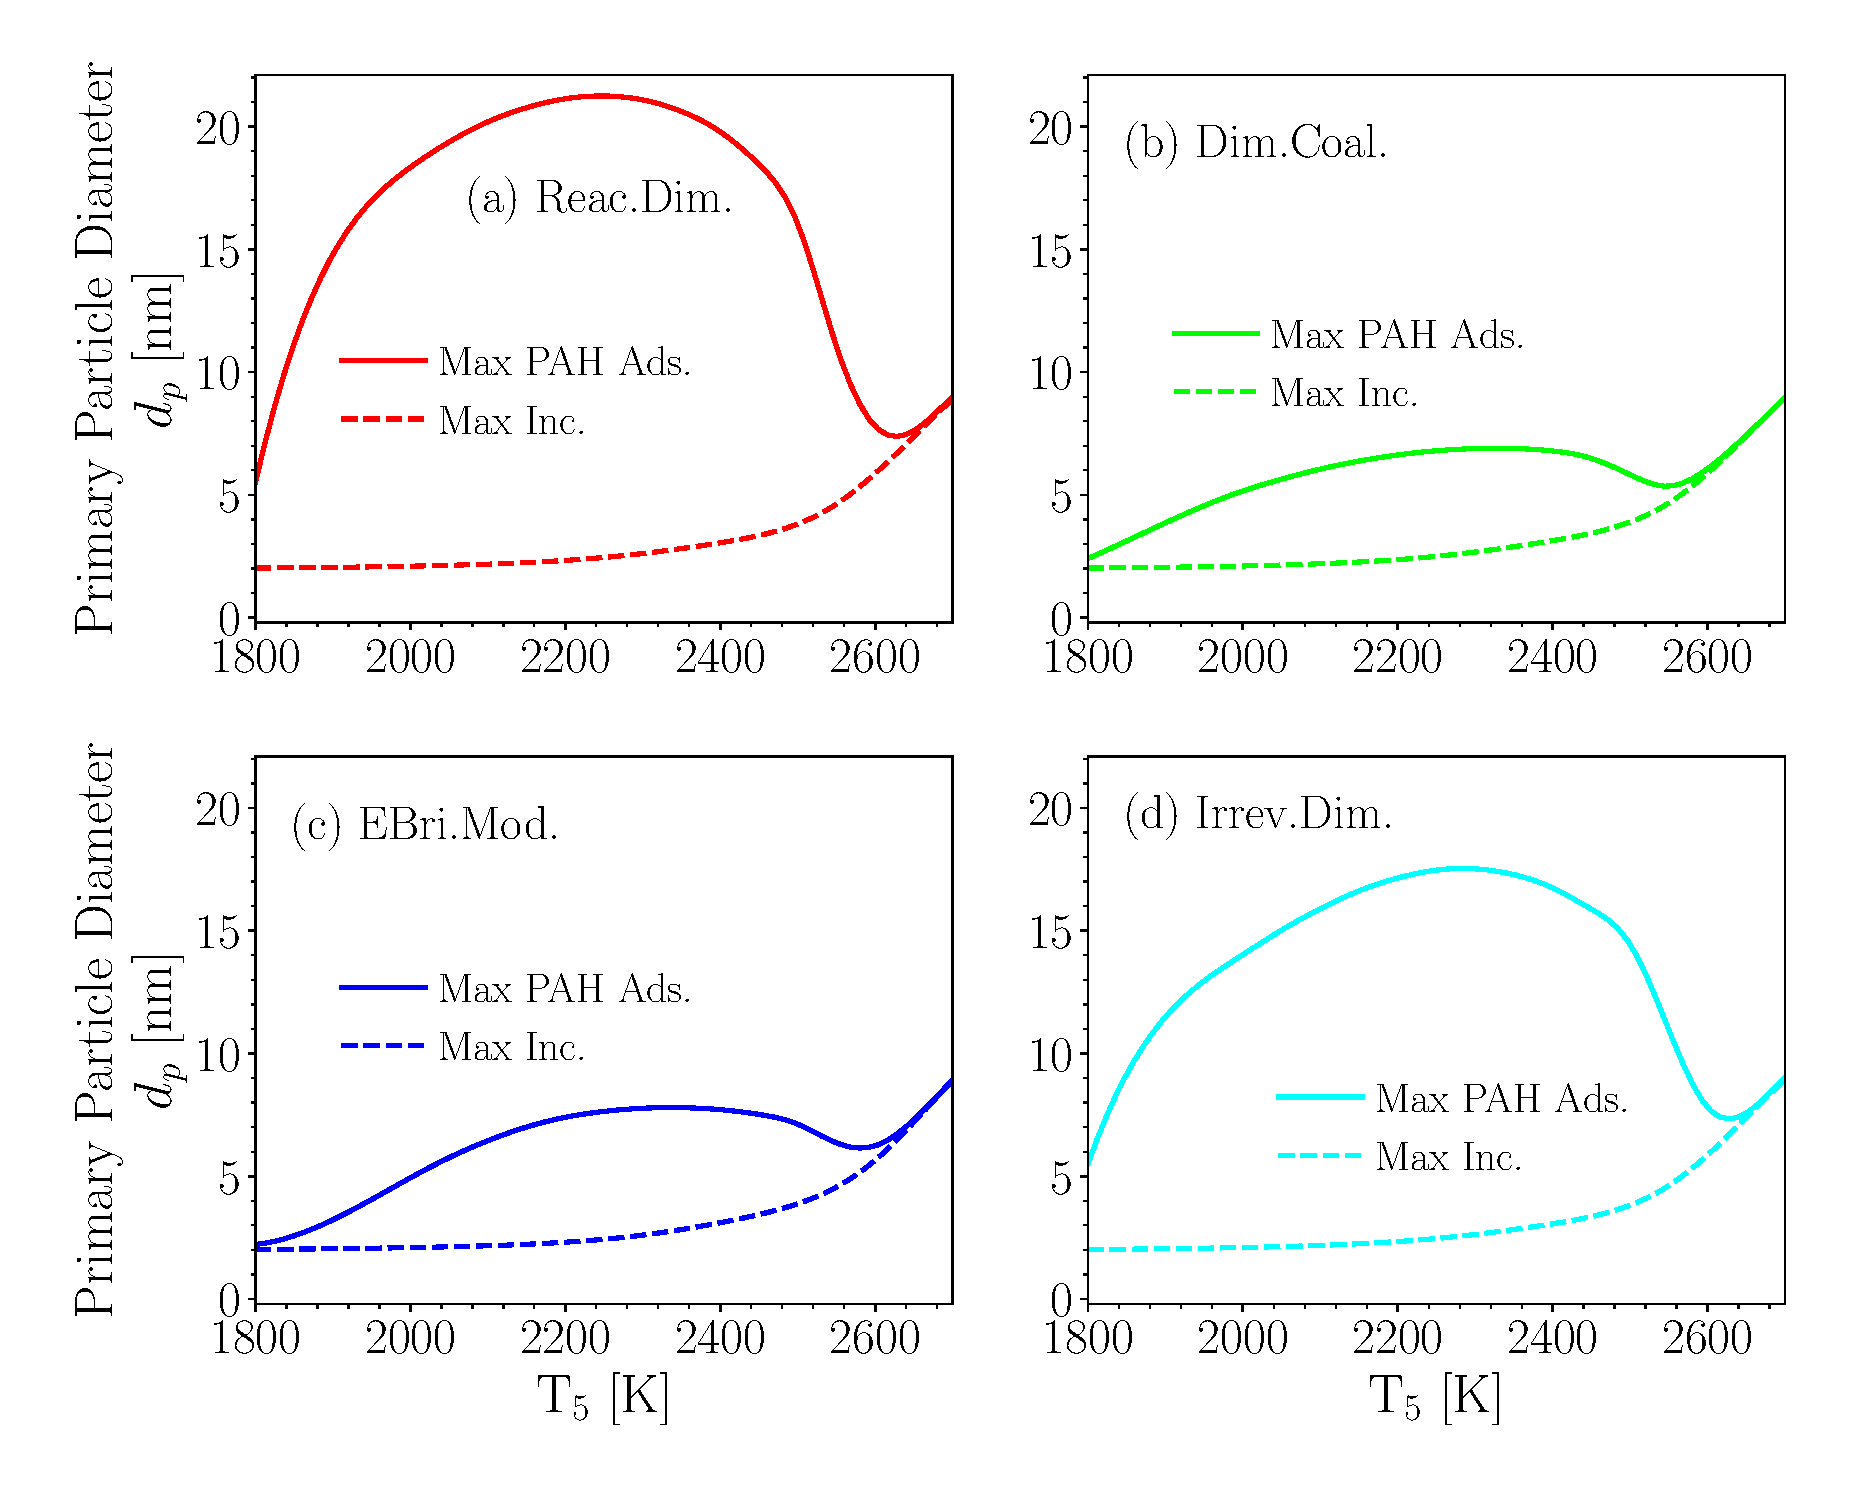
\includegraphics[width=0.8\textwidth]{Figures/Results/Shocktube/Agafonov2016/d_p_maxincads.pdf}
	\caption{The comparison of mean primary particle, $d_p$ at t=1.5 ms when maximum inception and PAH adsorption were applied to minimized the prediction  error compared to measurements~\citep{agafonov2016unified} for 5\% (a) and 10\%~$\mathrm{CH_4}$ (b) in Ar obtained using Caltech mechanism and different inception models.}
	\label{fig:shockagof_dp_maxincads} 
\end{figure}